
\documentclass{article}
\usepackage[headheight=20pt, margin=1.0in, top=1.2in]{geometry}
\usepackage{amsmath, amssymb, amsthm, thmtools, tcolorbox, array, graphicx, makeidx, cancel, multirow, fancyhdr, xypic, color, nicefrac, rotating, multicol, caption, subcaption, xcolor, tikz, tikz-3dplot, tikz-cd, pgfplots, import, enumitem, calc, booktabs, wrapfig, siunitx, hyperref,float}
\hypersetup{colorlinks=true,linkcolor=blue}
\usepackage[all]{xy}
\usepackage{esint}
\setlength{\parindent}{0in}
\sisetup{per-mode = symbol}
\usetikzlibrary{calc,arrows,svg.path,decorations.markings,patterns,matrix,3d,fit}
\usepgfplotslibrary{groupplots}
\pgfplotsset{compat=newest}
\newtcolorbox{mydefbox}[2][]{colback=red!5!white,colframe=red!75!black,fonttitle=\bfseries,title=#2,#1}
\newtcolorbox{mythmbox}[2][]{colback=gray!5!white,colframe=gray!75!black,fonttitle=\bfseries,title=#2,#1}
\newtcolorbox{myexamplebox}[2][]{colback=green!5!white,colframe=green!75!black,fonttitle=\bfseries,title=#2,#1}
\newtcolorbox{mypropbox}[2][]{colback=blue!5!white,colframe=blue!75!black,fonttitle=\bfseries,title=#2,#1}
\declaretheoremstyle[headfont=\color{blue}\normalfont\bfseries,]{colored}
\theoremstyle{definition}
\newtheorem{theorem}{Theorem}
\newtheorem{corollary}[theorem]{Corollary}
\newtheorem{lemma}[theorem]{Lemma}
\newtheorem{proposition}[theorem]{Proposition}
\newtheorem{problem}[theorem]{Problem}
\newtheorem{definition}[theorem]{Definition}
\newtheorem{exercise}[theorem]{Exercise}
\newtheorem{example}[theorem]{Example}
\newtheorem{solution}[theorem]{Solution}
\newtheorem*{thm}{Theorem}
\newtheorem*{lem}{Lemma}
\newtheorem*{prob}{Problem}
\newtheorem*{exer}{Exercise}
\newtheorem*{prop}{Proposition}
\def\R{\mathbb{R}}
\def\F{\mathbb{F}}
\def\Q{\mathbb{Q}}
\def\C{\mathbb{C}}
\def\N{\mathbb{N}}
\def\Z{\mathbb{Z}}
\def\Ra{\Rightarrow}
\def\e{\epsilon}
\newcommand{\typo}[1]{{\color{red}{#1}}}
\newcommand\thedate{\today}
\newcommand{\mb}{\textbf}
\newcommand{\norm}[2]{\|{#1}\|_{#2}}
\newcommand{\normm}[1]{\|#1\|}
\newcommand{\mat}[1]{\begin{bmatrix} #1 \end{bmatrix}}
\newcommand{\eqtext}[1]{\hspace{3mm} \text{#1} \hspace{3mm}}
\newcommand{\set}[1]{\{#1\}}
\newcommand{\inte}{\textrm{int}}
\newcommand{\ra}{\rightarrow}
\newcommand{\minv}{^{-1}}
\newcommand{\tx}[1]{\text{ {#1} }}
\newcommand{\abs}[1]{|#1|}
\newcommand{\mc}[1]{\mathcal{#1}}
\newcommand{\uniflim}{\mathop{\mathrm{unif\lim}}}
\newcommand{\notimplies}{\mathrel{{\ooalign{\hidewidth$\not\phantom{=}$\hidewidth\cr$\implies$}}}}
\pagestyle{fancy}
\fancyhf{}
\fancyhead[L]{Title of the Document}
\fancyhead[C]{}
\fancyhead[R]{\thepage}
\fancyfoot[L]{}
\fancyfoot[C]{}
\fancyfoot[R]{}
\renewcommand{\headrulewidth}{0.4pt}
\renewcommand{\footrulewidth}{0.4pt}
\numberwithin{equation}{section}
% Increase spacing between paragraphs
\setlength{\parskip}{1em}
% Increase spacing before and after sections
\usepackage{titlesec}
\titlespacing*{\section}{0pt}{3ex plus 1ex minus .2ex}{2ex plus .2ex}
\titlespacing*{\subsection}{0pt}{2ex plus 1ex minus .2ex}{1ex plus .2ex}
\titlespacing*{\subsubsection}{0pt}{1ex plus 1ex minus .2ex}{1ex plus .2ex}
\title{\textbf{Title of the Document}}
\author{Author Name}
\date{\today}
\begin{document}
\maketitle
\tableofcontents
\newpage
\section*{2.6 Exercises}
\begin{itemize}
    \item[2-1.] Let $(X,d)$ be a metric space and $S \subseteq X$. Show that $\partial S \subseteq S'^c$.
    \item[2-2.] Show that for an arbitrary choice of $a,b,r \in \mathbb{R}$, the closed disk $(x-a)^2 + (y-b)^2 \leq r^2$ is a bounded set in $\mathbb{R}^2$.
    \item[2-3.] Let $(X,d)$ be a metric space and for $x,y \in X$. Show that if $d(x,y) < \epsilon$ for every $\epsilon > 0$, then $x = y$.
\end{itemize}

\begin{proof}[2-1]
Assume $\partial S \subseteq S'^c$. Therefore, there exists $x \in S'$ such that $x \in S$ which is a contradiction.\\
Then by $x \in S'^c$, $\exists \epsilon > 0 : B_\epsilon(x) \subseteq S'^c$.\\
However, by $x \in S'$, this value of $\epsilon > 0$ implies $B_\epsilon(x) \cap S \neq \emptyset \Rightarrow B_\epsilon(x) \subseteq S$, which is a contradiction, implying our assumption that $x \in \partial S \cap S'$ must be false, and $S' \cap S^{\text{int}}\!=\!\emptyset\!\Box$.
\end{proof}

\begin{proof}[2-2]
A set $S$ is bounded iff $\exists M \in \mathbb{R}^+$ s.t. $\forall x,y \in S$, $d(x,y) \leq M$. Let $a,b,r \in \mathbb{R}$.\\
$\delta = \{(x,y) \in \mathbb{R}^2| (x-a)^2 + (y-b)^2 \leq r^2 \}$
$
\Rightarrow x^2 - 2ax + a^2 + y^2 - 2yb + b^2 \ \leq \ r^2 \\
\Rightarrow x^2 - 2ax + y^2 - 2yb \ \leq \ r^2 - a^2 - b^2
$
$
\Rightarrow x^2 + y^2 \ \leq \ r^2 - a^2 - b^2 + 2xa + 2yb
$
\emph{Need to show} $x^2$ is bounded.\\
$(x-a)^2 \leq r^2$\\
$\Rightarrow \vert x - a \vert \leq \vert r \vert$\\
$\Rightarrow \vert x - a \vert + \vert a \vert \leq \vert r \vert + \vert a \vert$\\
$\Rightarrow \vert x \vert = \vert x - a + a \vert \leq \vert x - a \vert + \vert a \vert \leq r + a \vert$.
\end{proof}

% Diagram of a circle with a radius a and b with `L` labeled and `|x| ≤ r + |a|`
\begin{figure}[h!]
\centering
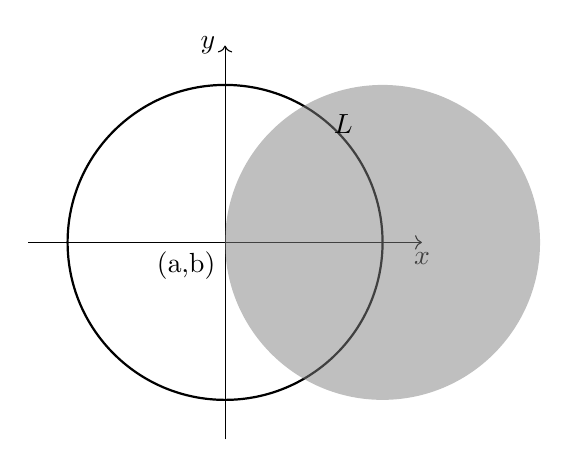
\begin{tikzpicture}
\draw[thick] (0,0) circle(2cm);
\draw[->] (-2.5,0) -- (2.5,0) node[anchor=north] {$x$};
\draw[->] (0,-2.5) -- (0,2.5) node[anchor=east] {$y$};
\fill[gray,opacity=0.5] (2,0) circle(2cm);
\node at (0,0) [anchor=north east] {(a,b)};
\node at (1.5,1.5) {$L$};
\end{tikzpicture}
\caption{A circle with radius $a$ and central point $(a,b)$}
\end{figure}

\Rightarrow |y| \le r + |a|

\Rightarrow y^2 \le (r + |a|)^2

\text{Same for } y, \quad y^2 \le (r + |b|)^2

\forall z=(x,y) \in D_{a,b}^2

\|z\| = \sqrt{x^2 + y^2} 

\le \sqrt{(r+|a|)^2+(r+|b|)^2}

\text{Thus if } M = \sqrt{(r+|a|)^2 + (r+|b|)^2}, \text{the bound holds.}

\# 15 \text{ normed boundedness = distance boundedness.}

\text{Let } x=(x_1,x_2), \; y=(y_1,y_2) \in D_{a,b}

z_1=(x_1,y_1)
(z_1 - a)^2 + (z_2 - b)^2 = r^2 

\Rightarrow d(z_1,(a,b)) = \sqrt{(x_1 - a)^2+(x_2 - b)^2} \le r

\Rightarrow d(x,y) \le d(x, (a,b)) + d(y, (a,b))

= \sqrt{(x_1 - a)^2+(x_2 - b)^2} + \sqrt{(y_1 - a)^2+(y_2 - b)^2}

\le r + r = 2r.

\begin{enumerate}
    \item[(iii)] \textbf{Suppose that} \(x \neq y\). \textbf{Then} \(d(x,y) \neq 0\). \textbf{Thus if we choose} \(\epsilon = d(x,y) \Rightarrow \epsilon > 0 \) \textbf{but} \(d(x,y) \geq \epsilon\). \emph{(contradiction).}

    \textbf{(contradiction) Suppose} \(x = y\) \textbf{and so} \(d(x,y) = 0 \).

    \textbf{Choose} \(\epsilon > 0 \) \textbf{so that}  \(\epsilon = d(x,y) \). \textbf{Then we must have} \(d(x,y) < \epsilon = \frac{d(0,0)}{2}\), \textbf{which is a contradiction, as this implies}

    $ \textbf{if} \ d(x,y) > 0 \ \textbf{so} \ d(x,y) = s < \epsilon = \frac{s}{2}$

    $ \Rightarrow s < \frac{s}{2} \Rightarrow 2s < s$

    \textbf{Thus}, \( x = y \).

    \item[(iv)] \textbf{Let} \((V, || \cdot ||) \ \textbf{be a normed vsp.} \)

    \textbf{Then let} \( \ r > 0 \ \textbf{and} \ x \in V \).

    $ B_r(x) = \{y \in V \ | \ d(x,y) < r \} $
    $ B_{r + ||x||}(0) = \{y \in V \ | \ d(0,y) < r + ||x||\} $

    \textbf{Let} \( y \in B_r(x)\).

    $
        d(0,y) \leq d(0,x) + d(x,y)
        \leq ||x|| + r
        \Rightarrow B_r(x) \subseteq B_{r + ||x||}(0).
    $

    \item[(v)] \textbf{Suppose} \( S \ \textbf{is bounded.Then} \ \exists M \in \mathbb{R} : \forall x \in S \  ||x|| \leq M \).

    $
        \text{(Equiv to} \  \exists M \in \mathbb{R} : \forall x \in S \ x \in B_{M}(0)).
    $
\end{enumerate}\end{document}